\begin{center}
\LARGE{Messprotokoll}
\end{center}

The oszilloscope is connected to the output of the PMs of the scintillators and signals of roughly 50 to 500mV can be observed, whereas really big pulses dont occur very frequently. In Fig. \ref{Fig_1} one can see a typical pulse of the scintillator. Changing the terminating resistor from 50$\Omega$ to 1M$\Omega$ does not have a huge impact on the observed pulses, it does give a little overshoot after the pulse gets back to zero though (See Fig. \ref{Fig_2}). 

\begin{enumerate}
\item How are photons detected in a photomultiplier?\\
\item How are the photons generated in the scintillator?\\
The answers to the last two questions can be found in section 3 from above.
\item How much energy do relativistic particles such as muons from cosmic radiation deposit in a scintillator?\\
That depends on the type of scintillator. The mean energy that is lost by a high energy muon is described by the Bethe-Bloch equation (\ref{eq:bethebloch}).
\begin{equation} \label{eq:bethebloch}
	-\left\langle {\frac {dE}{dx}}\right\rangle ={\frac {4\pi }{m_{e}c^{2}}}\cdot {\frac {nz^{2}}{\beta ^{2}}}\cdot \left({\frac {e^{2}}{4\pi \varepsilon _{0}}}\right)^{2}\cdot \left[\ln \left({\frac {2m_{e}c^{2}\beta ^{2}}{I\cdot (1-\beta ^{2})}}\right)-\beta ^{2}\right]
}
\end{equation}
where $z$ is the charge, $E$ the energy, $x$ the distance the muon travels into a target of electron number density $n$ and mean excitation potential $I$, $c$ is the speed of light and $\epsilon_0$ the vacuum permittivity, $\beta=\frac{v}{c}$, $e$ and $m_e$ the electron charge and rest mass respectively. The energy dependence of the energy loss as described by Bethe-Bloch can be seen in Fig.\,\ref{f:bethebloch}\\ %TODO: Bethe-Bloch graph

For muons of energy 1 GeV we get $\beta\gamma\approx10$ which means that $\left\langle \frac{\mathrm{d}E}{\mathrm{d}x}\right\rangle \approx 2 \frac{\text{MeV}\cdot\text{cm}^2}{g}$. Unfortunately the exact scintillator type is not given. According to the Particle Data Group (\ref{pdg_scintillators}) densities for organic scintillators are around $1 \frac{\text{g}}{\text{cm}^3}	$ while densities for inorganic scintillators are in the range from $4-8 \frac{\text{g}}{\text{cm}^3}$. This means an energy loss of approximately $\left\langle \frac{\mathrm{d}E}{\mathrm{d}x}\right\rangle \approx 1-16 \frac{\text{MeV}}{cm}$. Since the scintillators are each 1cm thick, this is also the mean energyloss per scintillator plane. This loss is obvoiusly distributed around this mean value according to the Landau distribution. Also one has to note, that most muons that are used for the measurement are those, that decay inside the detector. As discussed above (TODO) these are very low energy muons, high energy muons (1GeV) will not be stopped by the detector. For minimum ionizing particles (MIPS), muons with $\beta\gamma\approx 3-4$ so energies of around 300-400MeV will probably deposit only about half this energy, whereas muons of even lower energies will deposit much more energy due to the rapid increase in energy loss below $\beta\gamma=3$.  
\item Which impact has the terminator on the waveform?\\
 \textbf{\LARGE{???TODO!!!}}
\item How do pulses from photomultiplier tubes look like?\\ 
A typical pulse from the photomultiplier (PMT) can be seen in Fig.\,\ref{Fig_1}
\item What determines the height of these pulses?\\
The heigth of these pulses depends on various parameters. Most importantly it depends on the number of photons, which is proportional to the energy loss in the scintillator (as discussed above) that hit the photocathode of the PMT. More primary photoelectrons will create a stronger signal. (The integrated signal should roughly be proportional to the number of primary photoelectrons). It also depends on the multiplicity of the PMT, which in turn depends on the voltage applied to the electrodes in the PMT as well as the number, type and geometry of the dynodes.
\end{enumerate}

Next the thresholds are changed and a lower threshold (absolute value, since the pulses are negative) yields a higher rate but also seems to give an output signal if there is no clear signal. A higher threshold on the other hand yields a lower rate of very high peaked signals. Thresholds of around -10mV seemed to be a good compromise. The pulse heigths still varied between 50 to 500mV. The signal of the discriminator was slightly shifted from the scintillatorsignal by around 80ns and had a width of around 102ns. 

\begin{enumerate}
\item What is the functionality of the discriminators?\\
The discriminators make sure, that the timing of the different signals is done consistantly \ref{discriminator}. If the time when the threshold is passed by a signal would be taken, higher signals would give a signal slightly earlier than lower signals, since the rise to the threshold is faster if the signal is higher. A constant fraction discriminator solves this problem in that it gives a signal in the moment when the signal is a certain fraction of its way up to the peak (under the condition, that the threshold is passed at all). Thus giving better timing of the signals, which is crutial for lifetime measurements.  
\item Which impact has changing the thresholds?\\
The impact of the thresholds is already discussed above. 
\end{enumerate}

The scintillators have a width of $32.5\pm0.5$cm and a length of $82\pm2$cm. The length was not easily measurable since it was not clear where the scintillator ended and the readout started. The top of the photomultipliers where measured to be at $9.5 \pm 0.5; 85.0 \pm 0.5; 76.0 \pm 0.5; 66.0 \pm 0.5; 56.5 \pm 0.5; 47.5 \pm 0.5; 37.5 \pm 0.5; 28.0 \pm 0.5$ above ground. 

The couting rates were found to be around 100Hz for the thresholds used as above. For measurements that had the layer above and below as a reference, the detection efficiency was measured (assuming, that a signal in the two reference plains at the same time that does not give a signal in the measured layer means that a signal should have been observed but hasn't) to be 96.6\% for scintillator 1, 96.2\% for scintillator 2, 96.1\% for scintillator 3 and 91.6\% for scintillator 4. The thresholds where kept at -10mV since changing them did not improve the efficiency for scintillator 4. 

After this the rates drastically changed, so that we recalibrated the thresholds to -10mV for scintillator 0, -10mV for scintillator 1, -15mV for scintillator 2, -17mV for scintillator 3, -15mV for scintillator 4 and -30 for scintillator 5.
This gave us rates of 124.5Hz for scintillator 0, 128.4Hz for scintillator 1, 119.8Hz for scintillator 2, 140.3Hz for scintillator 3, 122.4Hz for scintillator 4 and 113.2Hz for scintillator 5. With these we got efficiencies of 97.5 (sc.1), 96.5 (sc.2), 94.9 (sc.3), 95.4 (sc.4) respectively. \\
At these rates we expect a rate of random coincidences of around 
\begin{equation}
	R_{12} = R_1R_2\Delta t \approx 0.00144\text{Hz}
\end{equation}
which is only roughly 0.0012\% of all events and can therefore be neglected.
\\

\subsection{Measurement of the muon lifetime}
The LabView program Lebensdauer.vi is then started and run for two days to aquire data. It also gives some online histograms that show the number of hits in each of the layers, the number of slices per event (e.g. the number of time slots in which signals have been registered for the whole detector) as well as some overwiev over the daq-session (elapsed time, number of events etc.). It also gives a rough representation of the discriminator output signals of all detector planes in different time slots. \\
A muon decay will here be seen as a signal that crosses some detectorplanes (e.g. there is a signal in all of them at the same time) and an additional signal in the same (decay upwards) or the one below (decay downwards) the last layer that has been hit. A delayed signal above the last layer that has been hit is most likely an afterpulse. These afterpulses can unfortunately also create false signals with the same caracteristics as a muon signal which means the afterpulse spectrum has to be subtracted from the muon spectrum later on. All other signals will not be used for further analysis. \\

The data was then analysed using a prewritten C++ program. 
The only thing that had to be added was an improved method to get the afterpulses, that have been described above. A basic method was already done that looked at the events that had a muon going through all the layers. This means that a signal in any but the last detector planes (thsi counld be a decay upwards just below the last detector plane) is most likely an afterpulse. However one can improve on this by also looking at all the events and registering afterpulses for all the planes above the last one that has been hit. Since the thickness of the absorbing metals matches the average range of the electrons coming from the muon decay it is likely that these kind of signals are afterpulses and not from the muon. Also a function that finds decays downwards had to be implemented and can be seen below.
\begin{lstlistings}
int fp13Analysis::findDecayDownward(int timeBin){
    if ((nLayers - 1) == lastMuonLayer)
        return -1;
    if ((1 << (lastMuonLayer+1)) & detectorHitMask[timeBin])
        return lastMuonLayer;
	return -1;
}
\end{lstlistings}
%% TODO: CODE einfügen
The more general function for the after pulses can be seen below.
\begin{lstlistings}
int fp13Analysis::findAfterpulsesImproved(int timeBin, int startLayer) {
    if (-1 == startLayer) 
    	startLayer = lastMuonLayer;
    for (int iLayer = startLayer -1 ; iLayer >= 0; iLayer--) {
        if ((1 << iLayer) & detectorHitMask[timeBin]) 
        	return iLayer;
    }
	return -1;
}
\end{lstlistings}

The program is then excecuted as described in the manual, which automatically fills several histograms. As described above afterpulses can also wrongly be identified as muon decays which means that the afterpulse spectrom has to be subtracted from the muon spectrum. To get the correct lifetime. 
The number of actual muons which decay upwards is given by
\begin{equation}
	N_\mu^0=N_{tot}-s\cdot N_{NP} = N_{tot} - \frac{N_{i,stop}}{N_{NP,start}}\cdot N_{NP}
\end{equation}
where $N_{tot}$ is the total number of muon candiates, $N_{i,stop}$ the number of signal events which only give signal until layer i, $N_{NP,start}$ the number of events that have been analysed for afterpulses and $N_{NP}$ the number of after pulses. The ratio $\frac{N_{NP}}{N_{NP,start}}$ therefore describes the probability that after the passage of a particle, an after pulse was produced. Since $N_{tot}$ and $N_{NP}$ depend on the decay time, the scaling factor $s = \frac{N_{i,stop}}{N_{NP,start}}$ is calculated to subtract the afterpulse spectrum from the muon candidates. The scaling factors can be seen in Tab.\,\ref{t:scaling}. For the decays downwards it is a little bit more complicated. For a decay down candidate to be an afterpulse, it is necessary that the muon should have produced a signal in the plane that is the same as the afterpulse but didnt register. This is described by the efficiency that has been determined above. The scaling factor is then given by $s = \frac{N_{i-1,stop}}{N_{NP,start}}\cdot\frac{1-\epsilon}{\epsilon}$, where $\epsilon$ is the efficnency. The error of the scaling factor (will be important later on for the up decay) is given by $\delta_s = s\sqrt{\frac{1}{N_{stop}}+\frac{1}{N_{start}}}$ since $N_{stop}$ and $N_{start}$ can be assumed to be poisson distributed. 
 
\begin{figure}
\begin{tabularx}{\textwidth}{| c | c | c | c | c |}
Location (Layer) & $N_{stop}$ & $N_{start}$ & Scaling factor s (up) & Error $\delta_s $ & Scaling factor s (down) \\
\hline
1 & 687990 & 1917633 & 0.3588 & 0.0005 & undefined\\
2 & 476842 & 1440791 & 0.3310 & 0.0006 & 0.0168\\
3 & 336548 & 1104243 & 0.3048 & 0.0006 & 0.0171\\
4 & 248892 & 855351 & 0.2910 & 0.0007 & 0.0160\\
5 & 855351 & 0 & undefined & undefined & undefined
\end{tabularx}
\caption{Scaling factor for the correction for the after-pulses histogram.}
\end{figure}

This corrected spectrum for the second detector plane can be seen in Fig.\,\ref{f:CorrectedMuons_new}

\begin{figure}
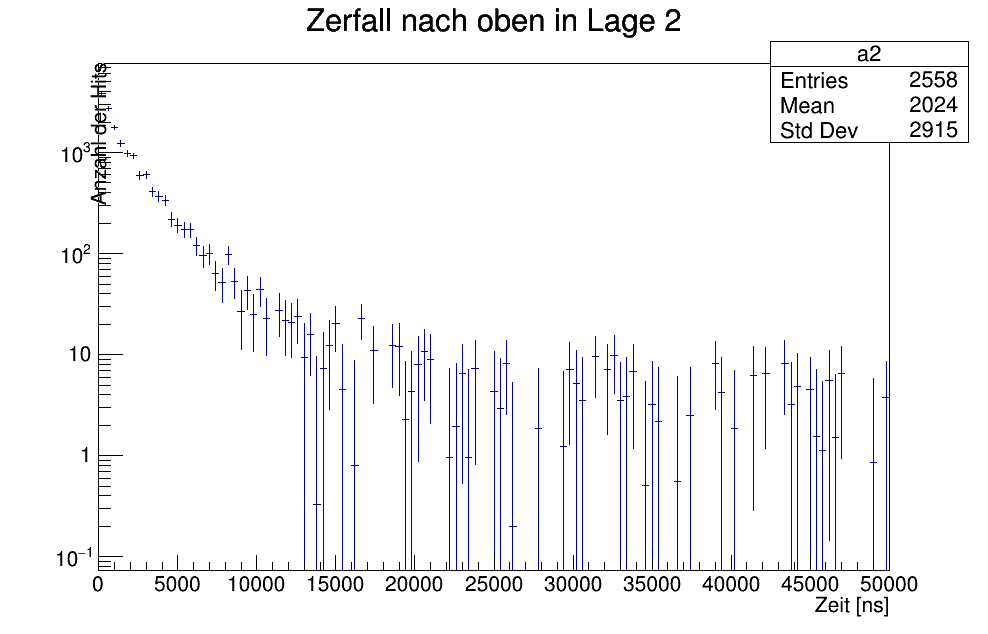
\includegraphics{CorrectedMuons_new.png}
\label{f:CorrectedMuons_new}
\end{figure} %TODO: Formatting

In Fig.\,\ref{f:lebensdauer_plots} one can see the different spectra for the different detector planes. 

%TODO: Add Lebensdauer:plots

The given macro Weiteres.C was analysed, no unexpected behaviour was observed. Fig.\ref{h3,h4}. %TODO



To this data we now fit a function of the form
\begin{equation} \label{eq:fit1}
	N(t)=N(\mu)e^{-\frac{t}{\tau_0}}+N_{BG}.
}
\end{equation}
This fit gives significantly different lifetimes depending on the fitrange as can be seen in Tab.\,\ref{t:lebensdauer}.
\begin{figure}
\begin{tabularx}{\textwidth}{| c | c | c | c | c | c |}
Measured quantity & 1000 - 20000 & 300 - 40000 & 300 - 20000 & 1000 - 40000 & 2000 - 40000\\
$\tau_0$ (up) & $1.93\pm 0.04$ & $1.87\pm0.04$ & $1.74\pm0.04$ & $2.09\pm0.05$ & $2.50\pm0.08$ \\
$\chi^2_{red}$ (up) & 2.2 & 3.5 & 4.0 & 2.3 & 1.6 \\
$\tau_0$ (down) & $1.91 \pm 0.05$ & $1.91\pm0.04$ & $1.86\pm0.04$ & $1.97\pm0.05$ & $2.21\pm0.08$ \\
$\chi^2_{red}$ (down) & 1.9 & 1.4 & 2.0 & 1.4 & 1.1 \\
$\tau_0$ (combined) & $1.93\pm0.04$ & $1.88\pm 0.03$ & $1.76\pm0.03$ & $2.07 \pm0.04$ & $2.44\pm0.06$ \\
$\chi^2_{red}$ (combined) & 2.6 & 3.9 & 4.6 & 2.6 & 1.7 
\end{tabularx}
\caption{Fits for different Fitranges using Fit \ref{eq:fit1}.}
\label{t:lebensdauer}
\end{figure}
The plots to these fits can be seen in Fig.\,\ref{f:lebensdauer}
%TODO: Lebensdauer Plots (5 Stück) 

To take into account that the negative muons can also be captured by atoms one has to modify the fit function slightly to
\begin{equation} \label{eq:fit2}
	N(t)=N_{\mu^+}\cdot e^{-\frac{t}{\tau_0}}\left(\frac{1}{f}e^{-\frac{t}{\tau_C}}+1\right)+N_{BG}
\end{equation}
where f is the ratio $\frac{N_{\mu^+}}{N_\mu^-}$. 

Again the lifetime was quite dependent on the fitrange, the results can be seen in Tab.\,\ref{t:einfangzeiten}

\begin{figure}
\begin{tabularx}{\textwidth}{| c | c | c | c | c | c |}
Measured quantity & 1000 - 20000 & 300 - 40000 & 300 - 20000 & 1000 - 40000 & 2000 - 40000\\
$\tau_0$ (up) & $2.20\pm0.07$ & $2.16\pm0.05$ & $2.00\pm0.05$ & $2.40\pm0.06$ & $2.7\pm0.7  $ \\
$\tau_c$ (up) & $1.24\pm0.26$ & $1.00\pm0.13$ & $0.89\pm0.13$ & $1.43\pm0.21$ & $1.50\pm0.11$ \\
$\chi^2_{red}$ (up) & 1.5 & 2.3 & 2.2 & 1.7 & 1.4 \\
$\tau_0$ (down) & $2.20\pm0.07$ & $1.91\pm 0.04$ & $2.21\pm0.05$ & $2.26\pm0.07$ & $2.37\pm0.08$ \\
$\tau_c$ (down) & $1.34\pm0.31$ & $0.1\pm1.0$ & $1.38 \pm 0.27$  & $1.38\pm0.29$ & $1.5\pm0.9  $ \\
$\chi^2_{red}$ (down) & 1.4 & 1.5 & 1.4 & 1.1 & 1.0 \\
$\tau_0$ (combined) & $2.20\pm0.06$ & $2.17\pm0.04$ & $2.04\pm0.04$ & $2.37\pm0.05$ & $2.62\pm0.07$ \\
$\tau_c$ (combined) & $1.25\pm0.23$ & $1.03\pm0.12$ & $0.92\pm0.12$ & $1.42\pm0.19$ & $1.50\pm0.10$ \\
$\chi^2_{red}$ (combined) & 1.6 & 2.4 & 2.3 & 1.9 & 1.5
\end{tabularx}
\caption{Fits for different Fitranges using Fit \ref{eq:fit2}.}
\label{t:einfangzeiten}
\end{figure}
In Fig.\,\ref{f:einfangzeiten} one can see one typical graph from these fits. %TODO: Einfangzeitengraph einfügen


The parameter f was then changed to find out its systematic impact, the results can be seen in Tab.\,\ref{t:varf}
\begin{figure}
\begin{tabularx}{\textwidth}{| c | c | c | c | c | c |}
Measured quantity & $f=1.275$ & $f = 1.225$ & $f=1.325$ & $f = 1.175$ & $f = 1.375$\\
$\tau_0$ (combined) & $2.20\pm0.06$ & $2.21\pm0.06$ & $2.19\pm0.05$ & $2.22\pm0.06$ & $2.18\pm0.05$ \\
$\tau_c$ (combined) & $1.25\pm0.23$ & $1.25\pm0.22$ & $1.25\pm0.23$ & $1.25\pm0.22$ & $1.26\pm0.23$ \\
$\chi^2_{red}$ (combined) & 1.6 & 1.6 & 1.6 & 1.6 & 1.7
\end{tabularx}
\caption{Variation of Parameter f.}
\label{t:varf}
\end{figure}

The scaling factors are then systematically changed by $\pm1\sigma$, teh results can be seen in Tab.\,\ref{t:vars}
\begin{figure}
\begin{tabularx}{\textwidth}{| c | c | c | c | c | c |}
Measured quantity & $s' = s$  & $s' = s-1\sigma_s$ & $s' = s+1\sigma_s$ \\
$\tau_0$ (combined) & $2.20\pm0.06$ & $2.20\pm0.06$ & $2.20\pm0.06$ \\
$\tau_c$ (combined) & $1.25\pm0.23$ & $1.25\pm0.22$ & $1.25\pm0.23$ \\  
$\chi^2_{red}$ (combined) & 1.6 & 1.6 & 1.6
\end{tabularx}
\caption{Variation of Parameter the scaling factors.}
\label{t:vars}
\end{figure}

\subsection{Measurement of the muon polarisation}
Next a measurement with a magnetic field of 40mT parallel to the scintillator planes was applied and data is aquired over the weekend. As described above the muons are polarised, e.g. their spin is preferably downwards. This spin will now precess with the Larmor frequency. Because the decay of the muon is favoured to be in the direction of the spin, the counting rate should periodically change
\begin{equation}
	Z^{with}(t)=Z_0\cdot e^{-\frac{t}{\tau}}\cdot(1+P\cdot A\cdot\cos(\omega_{Larmor}\cdot t +\phi))
\end{equation}
if a magnetic field is present. Because the counting rate without a magntic field is given by 
\begin{equation}
	Z^{without}(t) = Z_0\cdot e^{-\frac{t}{\tau}}\cdot(1+P\cdot A\cdot\cos(\phi))
\end{equation}
we can look at 
\begin{equation}
	\frac{Z^{with}(t)-Z^{without}(t)}{Z^{with}(t)-Z^{without}(t)}\approx \frac{P\cdot A}{2}\cdot \cos(\omega_{Larmor}t+\phi)+c
\end{equation}
to eliminate the exponential decay and find the Larmorfrequency as well as the factor $P\cdot A$. 

For this the scaling factors first have to be recalculated for the new dataset, as can be seen in Tab.\,

\begin{figure}
\begin{tabularx}{\textwidth}{| c | c | c | c | c |}
Location (Layer) & $N_{stop}$ & $N_{start}$ & Scaling factor s (up) & Error $\delta_s$ & Scaling factor s (down)\\
\hline
1 & 1538400 & 4445981 & 0.3460 & 0.0003 & undefined\\
2 & 1065690 & 3380291 & 0.3153 & 0.0004 & 0.0165\\
3 & 769962 & 2610329 & 0.2950 & 0.0004 & 0.022\\
4 & 573869 & 2036460 & 0.2818 & 0.0004 & 0.0182\\
5 & 2036460 & 0 & undefined & undefined & undefined
\end{tabularx}
\caption{Scaling factor for the correction for the after-pulses polarisation measurement.}
\end{figure}

%expected Larmor frequency: 3.404 MHz

In Fig.\,\ref{f:asy} one can see the asymetry function including a fit for the relevant Parameters. Unfortunately the errorbars are so big, that the fit does not give a significant result for the Larmorfrequency. In Fig.\,\ref{f:asy_all} one can see the result it the afterpulse spectra are not subtracted from the muon spectra. Because they are present in both the spectra with a magnetic field as well as without they should cancel out and not have an effect on the outcome. This yields a much clearer result. 